\documentclass[a3paper,11pt]{article}
\usepackage[margin=25mm]{geometry}
\pagestyle{empty}
\usepackage{tikz}
\usetikzlibrary{arrows.meta,positioning,fit,calc}

\usepackage{pdflscape} % rotates that page in the PDF viewer
% ---------- Styles ----------
\tikzset{
    box/.style={
        draw,
        rounded corners,
        align=left,
        font=\small,
        inner sep=6pt,
        minimum width=52mm
    },
    title/.style={font=\bfseries\small},
    arrow/.style={-{Stealth[length=2.2mm]}, thick},
    dashedarrow/.style={-{Stealth[length=2.2mm]}, thick, dashed},
    group/.style={draw, rounded corners, inner sep=9pt}
}

\begin{document}
\begin{landscape}
	\begin{center}
		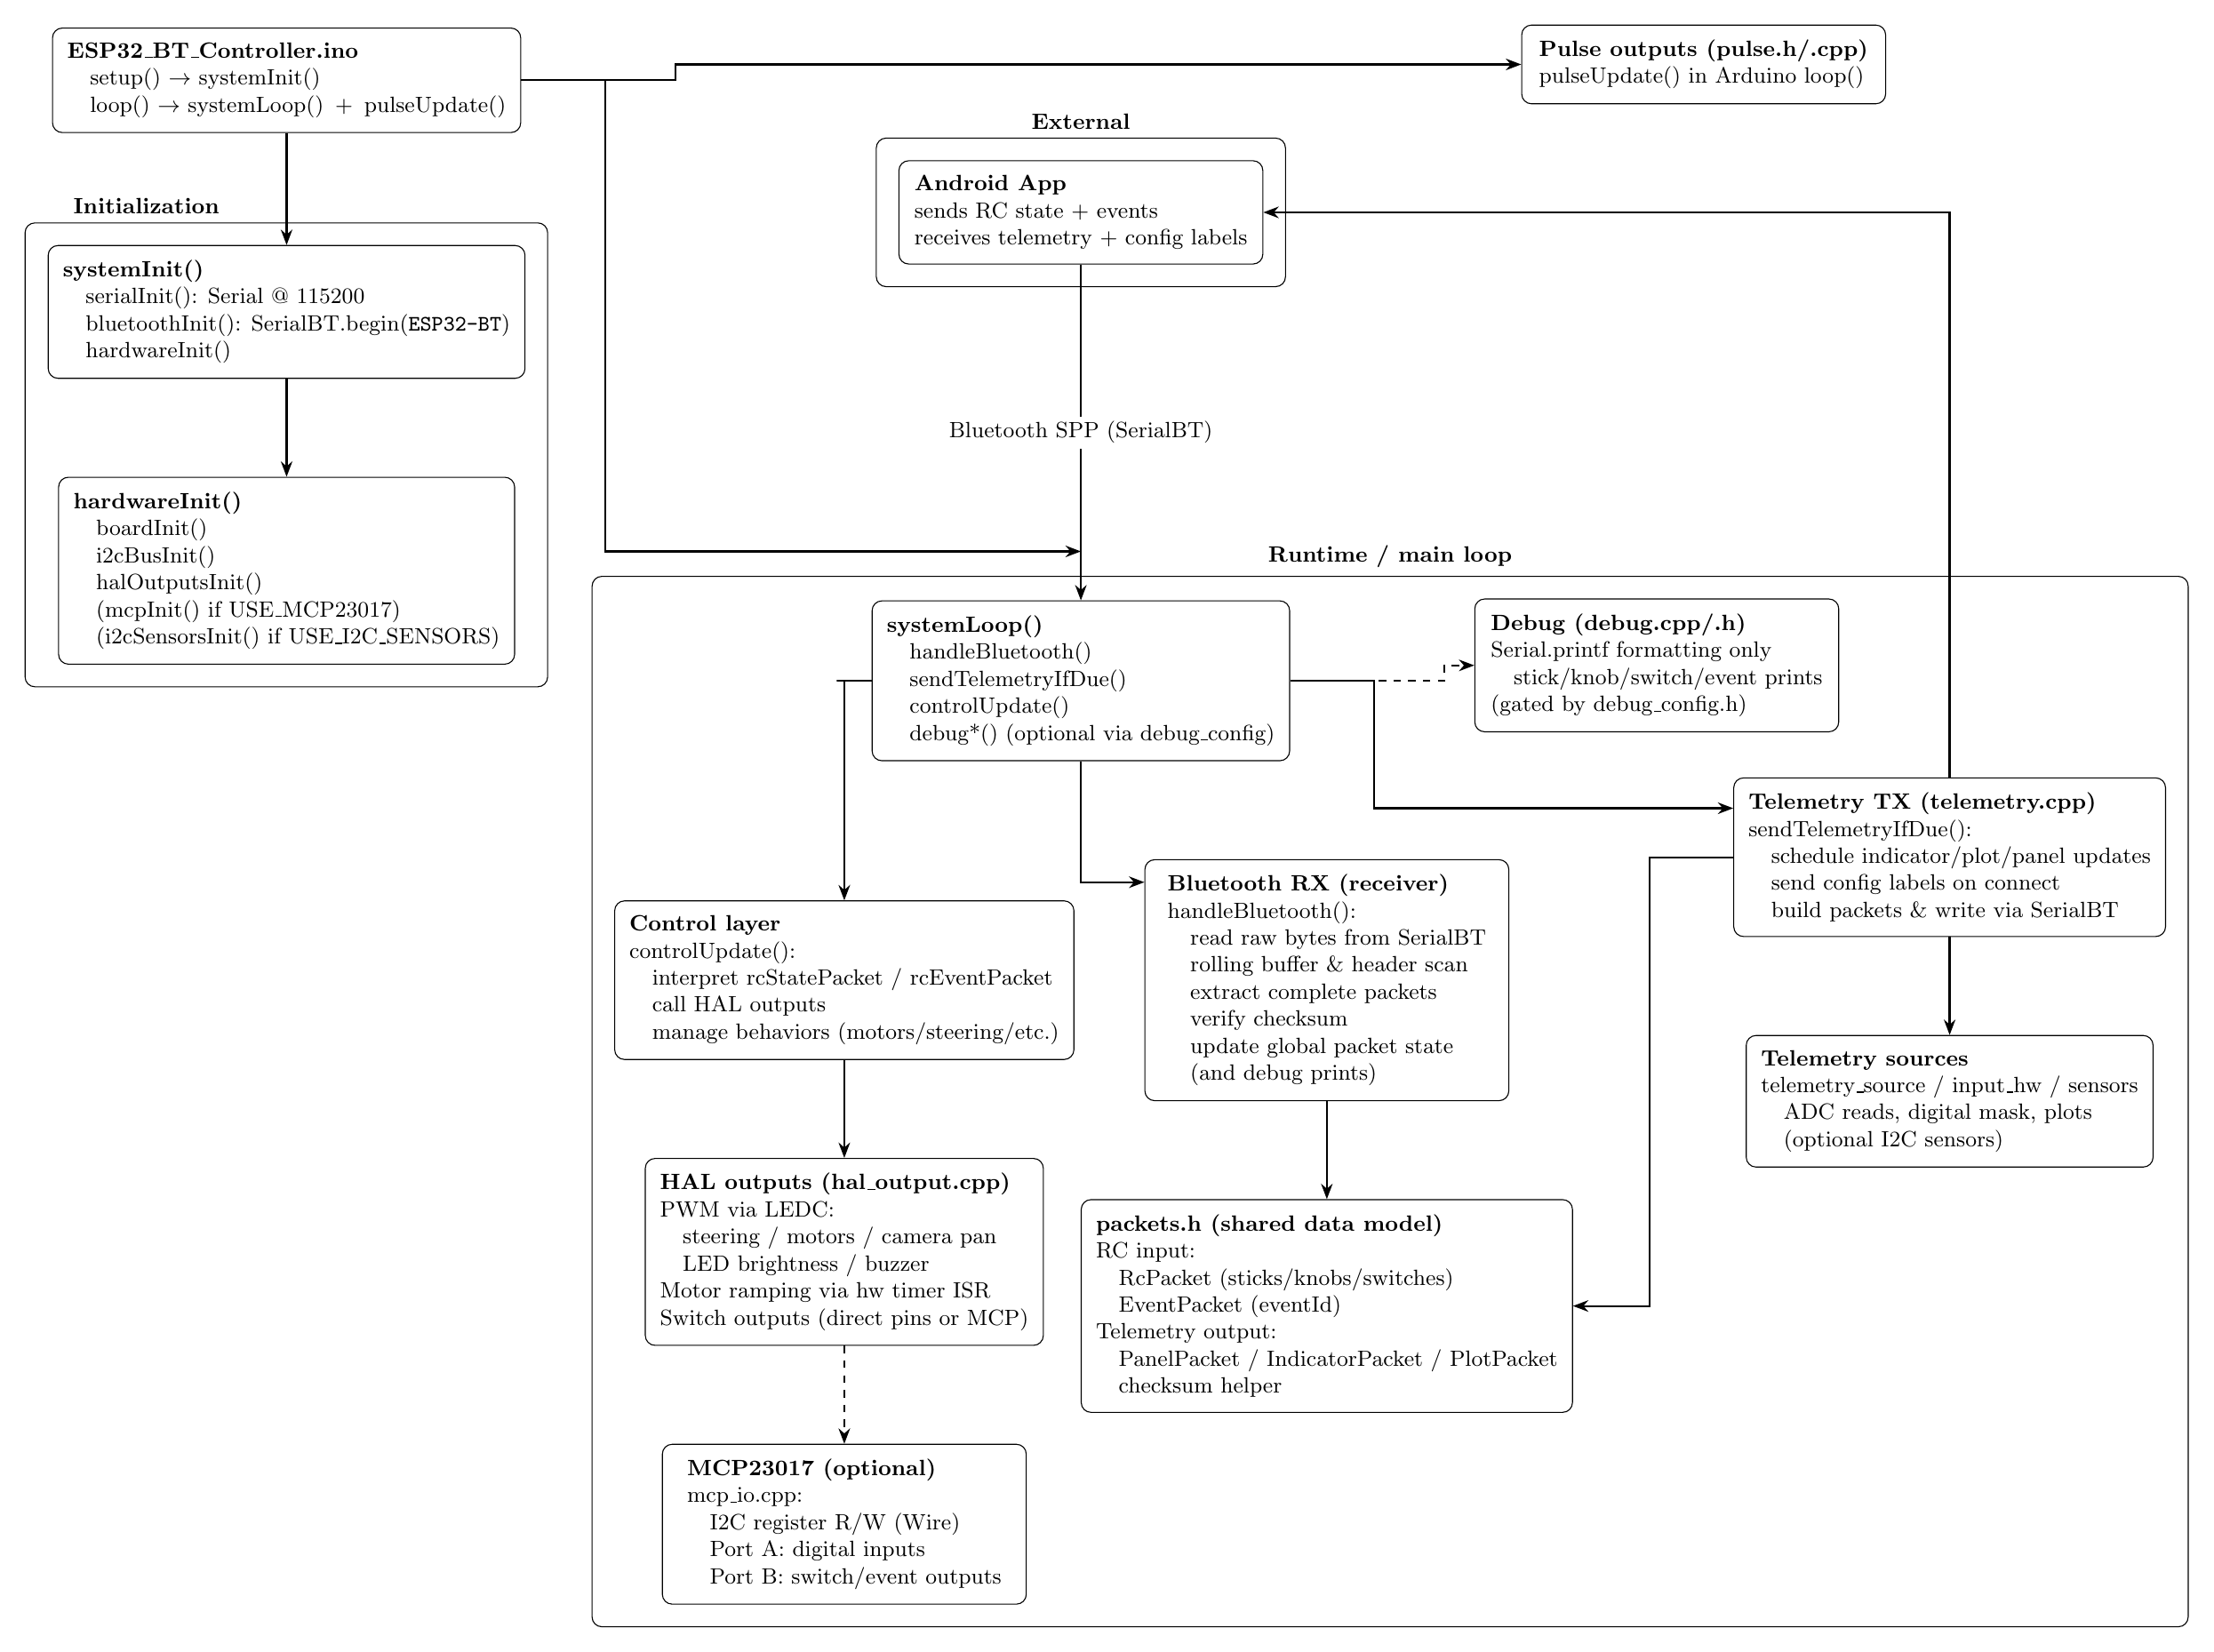
\begin{tikzpicture}[
				% Increase horizontal spacing aggressively to prevent overlap
				node distance=14mm and 38mm
			]

			% ======================================================
			% TOP: Entry points
			% ======================================================
			\node[box] (ino) {
			\textbf{ESP32\_BT\_Controller.ino}\\
			\quad setup() $\rightarrow$ systemInit()\\
			\quad loop() $\rightarrow$ systemLoop() \,+\, pulseUpdate()
			};

			% ======================================================
			% INIT AREA (left column under ino)
			% ======================================================
			\node[box, below=16mm of ino, anchor=north] (init) {
				\textbf{systemInit()}\\
				\quad serialInit(): Serial @ 115200\\
				\quad bluetoothInit(): SerialBT.begin(\texttt{ESP32-BT})\\
				\quad hardwareInit()
			};

			\node[box, below=14mm of init, anchor=north] (hw) {
				\textbf{hardwareInit()}\\
				\quad boardInit()\\
				\quad i2cBusInit()\\
				\quad halOutputsInit()\\
				\quad (mcpInit() if USE\_MCP23017)\\
				\quad (i2cSensorsInit() if USE\_I2C\_SENSORS)
			};

			% ======================================================
			% RUNTIME AREA (center column)
			% ======================================================
			\node[box, xshift=-30, yshift=-150, right=60mm of init, anchor=west] (loop) {
				\textbf{systemLoop()}\\
				\quad handleBluetooth()\\
				\quad sendTelemetryIfDue()\\
				\quad controlUpdate()\\
				\quad debug*() (optional via debug\_config)
			};

			\node[box, xshift=100, below=14mm of loop, anchor=north] (rx) {
				\textbf{Bluetooth RX (receiver)}\\
				handleBluetooth():\\
				\quad read raw bytes from SerialBT\\
				\quad rolling buffer \& header scan\\
				\quad extract complete packets\\
				\quad verify checksum\\
				\quad update global packet state\\
				\quad (and debug prints)
			};

			\node[box, below=14mm of rx, anchor=north] (packets) {
				\textbf{packets.h (shared data model)}\\
				RC input:\\
				\quad RcPacket (sticks/knobs/switches)\\
				\quad EventPacket (eventId)\\
				Telemetry output:\\
				\quad PanelPacket / IndicatorPacket / PlotPacket\\
				\quad checksum helper
			};

			% ======================================================
			% CONTROL / OUTPUTS (left of RX) -- push further left
			% ======================================================
			\node[box, left=10mm of rx, anchor=east] (control) {
				\textbf{Control layer}\\
				controlUpdate():\\
				\quad interpret rcStatePacket / rcEventPacket\\
				\quad call HAL outputs\\
				\quad manage behaviors (motors/steering/etc.)
			};

			\node[box, below=14mm of control, anchor=north] (hal) {
				\textbf{HAL outputs (hal\_output.cpp)}\\
				PWM via LEDC:\\
				\quad steering / motors / camera pan\\
				\quad LED brightness / buzzer\\
				Motor ramping via hw timer ISR\\
				Switch outputs (direct pins or MCP)
			};

			\node[box, below=14mm of hal, anchor=north] (mcp) {
				\textbf{MCP23017 (optional)}\\
				mcp\_io.cpp:\\
				\quad I2C register R/W (Wire)\\
				\quad Port A: digital inputs\\
				\quad Port B: switch/event outputs
			};

			% ======================================================
			% TELEMETRY (right of RX) -- push further right
			% ======================================================
			\node[box, yshift=50, right=32mm of rx, anchor=west] (telemetry) {
				\textbf{Telemetry TX (telemetry.cpp)}\\
				sendTelemetryIfDue():\\
				\quad schedule indicator/plot/panel updates\\
				\quad send config labels on connect\\
				\quad build packets \& write via SerialBT
			};

			\node[box, below=14mm of telemetry, anchor=north] (sources) {
				\textbf{Telemetry sources}\\
				telemetry\_source / input\_hw / sensors\\
				\quad ADC reads, digital mask, plots\\
				\quad (optional I2C sensors)
			};

			% ======================================================
			% DEBUG (far right) and PULSE (top of telemetry)
			% ======================================================
			\node[box, yshift=128,right=-5mm of rx, anchor=west] (debug) {
				\textbf{Debug (debug.cpp/.h)}\\
				Serial.printf formatting only\\
				\quad stick/knob/switch/event prints\\
				(gated by debug\_config.h)
			};

			\node[box, xshift=-100, yshift=222.5, above=18mm of telemetry, anchor=south] (pulse) {
				\textbf{Pulse outputs (pulse.h/.cpp)}\\
				pulseUpdate() in Arduino loop()
			};

			% ======================================================
			% EXTERNAL ACTOR (top of runtime)
			% ======================================================
			\node[box, above=48mm of loop, anchor=south] (android) {
				\textbf{Android App}\\
				sends RC state + events\\
				receives telemetry + config labels
			};

			% ======================================================
			% ARROWS (control flow)
			% ======================================================
			\draw[arrow] (ino) -- (init);
			\draw[arrow] (init) -- (hw);

			% ino -> loop (runtime entry)
			\draw[arrow] (ino.east) -- ++(12mm,0) |- ($(loop.north)+(0,7mm)$);

			% runtime chain
			\draw[arrow] (loop.south) |-($(rx.west)+(0,14mm)$);
			\draw[arrow] (rx) -- (packets);

			% loop -> control and outputs
			\draw[arrow] (loop.west) -- ++(-5mm,0) -| (control.north);
			\draw[arrow] (control) -- (hal);
			\draw[dashedarrow] (hal) -- (mcp);

			% loop -> telemetry
			\draw[arrow] (loop.east) -- ++(12mm,0) |- ($(telemetry.west)+(0,7mm)$);
			\draw[arrow] (telemetry) -- (sources);

			% packets used by telemetry (shared model)
			\draw[arrow] (telemetry.west) -- ++(-12mm,0) |- (packets.east);

			% debug depends on runtime state (optional)
			\draw[dashedarrow] (loop.east) -- ++(22mm,0) |- (debug.west);

			% pulse called from Arduino loop
			\draw[arrow] (ino.east) -- ++(22mm,0) |- (pulse.west);

			% ======================================================
			% Bluetooth links
			% ======================================================
			\draw[arrow] (android) -- node[midway,fill=white,inner sep=2pt]{\small Bluetooth SPP (SerialBT)} (loop.north);
			\draw[arrow] (telemetry.north) -- ++(0,72mm) |- (android.east);

			% ======================================================
			% GROUPING BOXES (fits)
			% ======================================================
			%        \node[group, fit=(init)(hw), label={[title]north:Initialization}] {};
			\node[draw=none, inner sep=0pt, minimum size=0pt] (init_fit_left)
			at ($(init.west)+(-0mm,0)$) {};

			% Put the label at a point on the top edge, shifted left by 20mm (tune as needed)
			% Draw the group box, but DON'T use label=...
			\node[group, fit=(init_fit_left)(init)(hw), name=initGroup] {};

			% Place the title manually, shifted left by 20mm (change to -50mm if you want)
			\node[title, anchor=south] at ($(initGroup.north)+(-20mm,0)$) {Initialization};
			\node[group, fit=(loop)(rx)(packets)(control)(hal)(mcp)(telemetry)(sources)(debug), label={[title]north:Runtime / main loop}] {};
			\node[group, fit=(android), label={[title]north:External}] {};

		\end{tikzpicture}
	\end{center}
\end{landscape}
% ======================================================
% Diagram explanation (for app users)
% ======================================================
\section{How the ESP32-BT Controller Works (Diagram Walkthrough)}
This section explains the architecture shown in the diagram from the point of view of an Android app user.
You do not need to understand the internal code to use the app, but this will help you understand what is
happening when you connect, move the sticks, or look at telemetry.

\subsection{Big picture}
The system is a Bluetooth ``remote control link'':

\begin{itemize}
	\item The \textbf{Android App} sends \textbf{control commands} (sticks, knobs, switches, and button events) to the ESP32.
	\item The \textbf{ESP32 firmware} receives those commands, converts them into \textbf{hardware outputs} (PWM, motors, LED, buzzer, switches), and optionally sends \textbf{telemetry} back to the app.
\end{itemize}

The firmware is organized into two phases:
\begin{enumerate}
	\item \textbf{Initialization} (runs once at power-on).
	\item \textbf{Runtime loop} (runs continuously as long as the ESP32 is powered).
\end{enumerate}

\subsection{Initialization phase (left group: ``Initialization'')}
When the ESP32 is powered on, the Arduino entry point \texttt{setup()} calls \texttt{systemInit()}.
This prepares everything needed for communication and hardware control:

\begin{description}
	\item[\texttt{serialInit()}] Starts the USB serial port at \texttt{115200}.
	      This is mainly for developer debug messages (it does not affect Bluetooth control).

	\item[\texttt{bluetoothInit()}] Starts classic Bluetooth SPP using \texttt{SerialBT.begin("ESP32-BT")}.
	      This is the Bluetooth device name your phone/app will see when scanning/pairing.

	\item[\texttt{hardwareInit()}] Initializes the hardware side:
	      \begin{itemize}
		      \item \texttt{boardInit()} sets up board-level pins/peripherals.
		      \item \texttt{i2cBusInit()} prepares the I\textsuperscript{2}C bus (if used).
		      \item \texttt{halOutputsInit()} prepares PWM timers / output pins.
		      \item Optional: \texttt{mcpInit()} if an MCP23017 expander is enabled (adds more digital I/O via I\textsuperscript{2}C).
		      \item Optional: \texttt{i2cSensorsInit()} if external sensors are enabled.
	      \end{itemize}
\end{description}

\subsection{Runtime phase (center group: ``Runtime / main loop'')}
After initialization, \texttt{loop()} runs forever. In this firmware, \texttt{loop()} calls:
\texttt{systemLoop()} (core logic) and \texttt{pulseUpdate()} (momentary button pulses).
This means your stick movement, switch toggles, and telemetry updates are processed continuously.

\subsection{Bluetooth receive path (``Bluetooth RX'')}
The Android app continuously sends small binary packets over Bluetooth.

\begin{itemize}
	\item The function \texttt{handleBluetooth()} reads raw bytes from \texttt{SerialBT}.
	\item It stores the bytes in a small rolling buffer.
	\item It searches for known packet headers (start markers) and only processes a packet when the full length is present.
	\item When a valid packet is found, it is copied into shared packet structures (described below).
\end{itemize}

\paragraph{What the app sends}
There are two main command types coming from the app:
\begin{description}
	\item[State packet (\texttt{RcPacket})] A ``full controller state'' snapshot:
	      left stick, right stick, two knobs, and a bitmask of switch states.
	      This is used for continuous control (steering, motor speed, pan, LED brightness, buzzer, etc.).

	\item[Event packet (\texttt{EventPacket})] A short ``button pressed'' message:
	      contains an \texttt{eventId}. This is used for momentary actions (pulse outputs).
\end{description}

\subsection{Shared packet model (``packets.h'')}
The diagram includes \texttt{packets.h} because it is the common language between modules:

\begin{itemize}
	\item RX writes into global packet variables (the most recent received data).
	\item Control reads from those packet variables to update outputs.
	\item Telemetry builds outgoing packets in fixed formats and writes them to Bluetooth.
\end{itemize}

In practical terms: if the app sends a new stick position, that data becomes the new ``current state'' used by
the control logic on every loop iteration.

\subsection{Control layer (``Control layer'')}
The control layer is where app commands turn into physical behavior.

\begin{itemize}
	\item \texttt{controlUpdate()} reads the latest values from the received state packet.
	\item It maps stick positions into PWM values.
	\item It calls the hardware abstraction layer (HAL) functions to apply those outputs.
\end{itemize}

\paragraph{Examples of what your controls do}
\begin{itemize}
	\item \textbf{Left stick X} $\rightarrow$ steering PWM.
	\item \textbf{Left stick Y} $\rightarrow$ left motor speed and direction.
	\item \textbf{Right stick X} $\rightarrow$ camera pan PWM.
	\item \textbf{Right stick Y} $\rightarrow$ right motor speed and direction.
	\item \textbf{Left knob} $\rightarrow$ LED brightness.
	\item \textbf{Right knob} $\rightarrow$ buzzer intensity.
	\item \textbf{Switches} $\rightarrow$ digital outputs (on/off).
\end{itemize}

\paragraph{Event buttons (momentary actions)}
When an event packet arrives, the receiver triggers \texttt{controlHandleEvent(eventId)}.
That function converts the event ID into a short pulse on one of the outputs (for example, ``press button 1''
may produce a short ON pulse on a particular output pin).

\subsection{HAL outputs (``hal\_output.cpp'')}
The HAL (hardware abstraction layer) is responsible for \textbf{writing to ESP32 hardware}:

\begin{itemize}
	\item Uses ESP32 LEDC PWM to generate servo/motor PWM signals.
	\item Drives direction pins for motors (forward/reverse).
	\item Implements motor ramping using a hardware timer interrupt, to smooth changes in speed.
	\item Controls switch outputs either:
	      \begin{itemize}
		      \item directly on ESP32 GPIO pins, or
		      \item through an optional MCP23017 I/O expander.
	      \end{itemize}
\end{itemize}

For the app user, this means: your UI controls directly translate into real electrical outputs on the ESP32 board.

\subsection{Optional MCP23017 (``MCP23017 (optional)'' box)}
If enabled, the MCP23017 provides additional digital I/O over I\textsuperscript{2}C.
The firmware can:
\begin{itemize}
	\item read digital inputs (e.g., indicators) from MCP Port A, and/or
	\item write outputs (switches/events) on MCP Port B.
\end{itemize}

\subsection{Telemetry transmit path (``Telemetry TX'')}
Telemetry is the opposite direction: ESP32 $\rightarrow$ Android App.

\begin{itemize}
	\item \texttt{sendTelemetryIfDue()} runs periodically inside \texttt{systemLoop()}.
	\item It only sends telemetry when the phone is connected (the firmware checks \texttt{SerialBT.hasClient()}).
	\item On a new connection it sends a \textbf{configuration message} (labels such as plot names and panel names),
	      so the app can automatically populate UI labels.
	\item It then sends periodic telemetry packets (panel, indicator, and plot values).
\end{itemize}

\paragraph{Telemetry sources}
The diagram shows a ``Telemetry sources'' box because telemetry does not invent values by itself.
It calls helper functions such as:
\begin{itemize}
	\item panel values (left/right),
	\item indicator values (analog + battery),
	\item plot values (three plot channels),
	\item optional sensor updates (if enabled).
\end{itemize}

So when you see changing telemetry on-screen, it is coming from these readings on the ESP32 side.

\subsection{Debug outputs (``Debug'' box)}
Debug output is for development and troubleshooting:
\begin{itemize}
	\item It prints formatted information to USB Serial.
	\item It can print sticks/knobs/switches/events depending on compile-time flags.
	\item It does not change control behavior; it only reports what is happening.
\end{itemize}

\subsection{Pulse outputs (``Pulse outputs'' box)}
Some app controls are ``momentary'' (press once, output a short pulse).
That behavior is handled by \texttt{pulseUpdate()}.

This ensures button presses behave like short taps rather than staying ON forever.

\subsection{What to check if something doesn’t work}
\begin{itemize}
	\item \textbf{Can’t connect:} verify the device appears as \texttt{ESP32-BT}, pair if required, and confirm Bluetooth is enabled.
	\item \textbf{Controls don’t respond:} connection may be present but packets aren’t arriving; verify the app is sending state updates.
	\item \textbf{Telemetry missing:} telemetry only transmits when a client is connected; also verify telemetry is enabled in the build.
\end{itemize}

% Note: This explanation is based on a code search view of the repo.
% GitHub code search results are limited and may be incomplete; if you add modules or change build flags,
% update this section accordingly.

\end{document}